\documentclass[twoside]{book}

% Packages required by doxygen
\usepackage{fixltx2e}
\usepackage{calc}
\usepackage{doxygen}
\usepackage[export]{adjustbox} % also loads graphicx
\usepackage{graphicx}
\usepackage[utf8]{inputenc}
\usepackage{makeidx}
\usepackage{multicol}
\usepackage{multirow}
\PassOptionsToPackage{warn}{textcomp}
\usepackage{textcomp}
\usepackage[nointegrals]{wasysym}
\usepackage[table]{xcolor}

% Font selection
\usepackage[T1]{fontenc}
\usepackage[scaled=.90]{helvet}
\usepackage{courier}
\usepackage{amssymb}
\usepackage{sectsty}
\renewcommand{\familydefault}{\sfdefault}
\allsectionsfont{%
  \fontseries{bc}\selectfont%
  \color{darkgray}%
}
\renewcommand{\DoxyLabelFont}{%
  \fontseries{bc}\selectfont%
  \color{darkgray}%
}
\newcommand{\+}{\discretionary{\mbox{\scriptsize$\hookleftarrow$}}{}{}}

% Page & text layout
\usepackage{geometry}
\geometry{%
  a4paper,%
  top=2.5cm,%
  bottom=2.5cm,%
  left=2.5cm,%
  right=2.5cm%
}
\tolerance=750
\hfuzz=15pt
\hbadness=750
\setlength{\emergencystretch}{15pt}
\setlength{\parindent}{0cm}
\setlength{\parskip}{3ex plus 2ex minus 2ex}
\makeatletter
\renewcommand{\paragraph}{%
  \@startsection{paragraph}{4}{0ex}{-1.0ex}{1.0ex}{%
    \normalfont\normalsize\bfseries\SS@parafont%
  }%
}
\renewcommand{\subparagraph}{%
  \@startsection{subparagraph}{5}{0ex}{-1.0ex}{1.0ex}{%
    \normalfont\normalsize\bfseries\SS@subparafont%
  }%
}
\makeatother

% Headers & footers
\usepackage{fancyhdr}
\pagestyle{fancyplain}
\fancyhead[LE]{\fancyplain{}{\bfseries\thepage}}
\fancyhead[CE]{\fancyplain{}{}}
\fancyhead[RE]{\fancyplain{}{\bfseries\leftmark}}
\fancyhead[LO]{\fancyplain{}{\bfseries\rightmark}}
\fancyhead[CO]{\fancyplain{}{}}
\fancyhead[RO]{\fancyplain{}{\bfseries\thepage}}
\fancyfoot[LE]{\fancyplain{}{}}
\fancyfoot[CE]{\fancyplain{}{}}
\fancyfoot[RE]{\fancyplain{}{\bfseries\scriptsize Generated by Doxygen }}
\fancyfoot[LO]{\fancyplain{}{\bfseries\scriptsize Generated by Doxygen }}
\fancyfoot[CO]{\fancyplain{}{}}
\fancyfoot[RO]{\fancyplain{}{}}
\renewcommand{\footrulewidth}{0.4pt}
\renewcommand{\chaptermark}[1]{%
  \markboth{#1}{}%
}
\renewcommand{\sectionmark}[1]{%
  \markright{\thesection\ #1}%
}

% Indices & bibliography
\usepackage{natbib}
\usepackage[titles]{tocloft}
\setcounter{tocdepth}{3}
\setcounter{secnumdepth}{5}
\makeindex

% Hyperlinks (required, but should be loaded last)
\usepackage{ifpdf}
\ifpdf
  \usepackage[pdftex,pagebackref=true]{hyperref}
\else
  \usepackage[ps2pdf,pagebackref=true]{hyperref}
\fi
\hypersetup{%
  colorlinks=true,%
  linkcolor=blue,%
  citecolor=blue,%
  unicode%
}

% Custom commands
\newcommand{\clearemptydoublepage}{%
  \newpage{\pagestyle{empty}\cleardoublepage}%
}

\usepackage{caption}
\captionsetup{labelsep=space,justification=centering,font={bf},singlelinecheck=off,skip=4pt,position=top}

%===== C O N T E N T S =====

\begin{document}

% Titlepage & ToC
\hypersetup{pageanchor=false,
             bookmarksnumbered=true,
             pdfencoding=unicode
            }
\pagenumbering{roman}
\begin{titlepage}
\vspace*{7cm}
\begin{center}%
{\Large Hubbard Model Exact Diagonalization }\\
\vspace*{1cm}
{\large Generated by Doxygen 1.8.11}\\
\end{center}
\end{titlepage}
\clearemptydoublepage
\tableofcontents
\clearemptydoublepage
\pagenumbering{arabic}
\hypersetup{pageanchor=true}

%--- Begin generated contents ---
\chapter{Hubbard model exact diagonalization}
\label{md_README}
\hypertarget{md_README}{}
References\+:


\begin{DoxyEnumerate}
\item H. Q. Lin, J. E. Gubernatis, Harvey Gould, and Tobochnik, computers in physics, 7,400(1993) 
\item S. A. Jafari, I\+J\+PR, 8,113,(2008)  
\end{DoxyEnumerate}
\chapter{Class Index}
\section{Class List}
Here are the classes, structs, unions and interfaces with brief descriptions\+:\begin{DoxyCompactList}
\item\contentsline{section}{\hyperlink{classbasis}{basis} }{\pageref{classbasis}}{}
\item\contentsline{section}{\hyperlink{classhamil}{hamil} }{\pageref{classhamil}}{}
\item\contentsline{section}{\hyperlink{classlhamil}{lhamil} }{\pageref{classlhamil}}{}
\item\contentsline{section}{\hyperlink{classMat}{Mat} }{\pageref{classMat}}{}
\item\contentsline{section}{\hyperlink{classTimer}{Timer} }{\pageref{classTimer}}{}
\item\contentsline{section}{\hyperlink{classVec}{Vec} }{\pageref{classVec}}{}
\end{DoxyCompactList}

\chapter{Class Documentation}
\hypertarget{classbasis}{}\section{basis Class Reference}
\label{classbasis}\index{basis@{basis}}
\subsection*{Public Member Functions}
\begin{DoxyCompactItemize}
\item 
{\bfseries basis} (long, long, long)\hypertarget{classbasis_ad982d3f0be65c05675cdc0efb00252a1}{}\label{classbasis_ad982d3f0be65c05675cdc0efb00252a1}

\item 
const \hyperlink{classbasis}{basis} \& {\bfseries operator=} (const \hyperlink{classbasis}{basis} \&)\hypertarget{classbasis_a0c6e641dfcb8827c4412e581fa4c8bfa}{}\label{classbasis_a0c6e641dfcb8827c4412e581fa4c8bfa}

\item 
long {\bfseries hopping\+\_\+up} (long, long, long)\hypertarget{classbasis_ad81055daddd429c17d3d8ec8df98c564}{}\label{classbasis_ad81055daddd429c17d3d8ec8df98c564}

\item 
long {\bfseries hopping\+\_\+down} (long, long, long)\hypertarget{classbasis_aabd03a8b22fc17da971a9cb9345a9ff9}{}\label{classbasis_aabd03a8b22fc17da971a9cb9345a9ff9}

\item 
long {\bfseries potential} (long, long, long)\hypertarget{classbasis_a64bb5f4caae7c3fc68bf788638c38276}{}\label{classbasis_a64bb5f4caae7c3fc68bf788638c38276}

\item 
long {\bfseries onsite\+\_\+up} (long, long)\hypertarget{classbasis_af150181d5a345a54732c7fe67b0dacc6}{}\label{classbasis_af150181d5a345a54732c7fe67b0dacc6}

\item 
long {\bfseries onsite\+\_\+down} (long, long)\hypertarget{classbasis_aaddb33fcac06a345845896b3f6114dbd}{}\label{classbasis_aaddb33fcac06a345845896b3f6114dbd}

\item 
long {\bfseries factorial} (long, long)\hypertarget{classbasis_a01aa1995b52a74c6415c123a8deceb83}{}\label{classbasis_a01aa1995b52a74c6415c123a8deceb83}

\item 
void {\bfseries init} ()\hypertarget{classbasis_ae335f2b871ce8fad7a5b8e3cab7c4f71}{}\label{classbasis_ae335f2b871ce8fad7a5b8e3cab7c4f71}

\item 
void {\bfseries generate\+\_\+up} (long)\hypertarget{classbasis_a35e25610628c2bb321c17a27537690b7}{}\label{classbasis_a35e25610628c2bb321c17a27537690b7}

\item 
void {\bfseries generate\+\_\+down} (long)\hypertarget{classbasis_aa8adf1b06de7d9c44f1554fc8c5afdf9}{}\label{classbasis_aa8adf1b06de7d9c44f1554fc8c5afdf9}

\item 
long {\bfseries creation} (long, long)\hypertarget{classbasis_a6d23794e33f4e4e4ac9836b16bd3745d}{}\label{classbasis_a6d23794e33f4e4e4ac9836b16bd3745d}

\item 
long {\bfseries annihilation} (long, long)\hypertarget{classbasis_a52c6f61e28d26ccb11a9cfca15eac18f}{}\label{classbasis_a52c6f61e28d26ccb11a9cfca15eac18f}

\item 
void {\bfseries prlong} ()\hypertarget{classbasis_af9ae0374ec02f33f9e3c10858172815a}{}\label{classbasis_af9ae0374ec02f33f9e3c10858172815a}

\end{DoxyCompactItemize}
\subsection*{Public Attributes}
\begin{DoxyCompactItemize}
\item 
long {\bfseries nsite}\hypertarget{classbasis_a98ef7e9fb8e86e6ca40f9356741d02b8}{}\label{classbasis_a98ef7e9fb8e86e6ca40f9356741d02b8}

\item 
long {\bfseries nel\+\_\+up}\hypertarget{classbasis_abb8238ae962d05c706adc219b9fb8102}{}\label{classbasis_abb8238ae962d05c706adc219b9fb8102}

\item 
long {\bfseries nel\+\_\+down}\hypertarget{classbasis_a90ff415d09d178ef397ede3613579148}{}\label{classbasis_a90ff415d09d178ef397ede3613579148}

\item 
map$<$ long, long $>$ {\bfseries basis\+\_\+up}\hypertarget{classbasis_a001c54b2d5cb432e2152bca56c9fcd4b}{}\label{classbasis_a001c54b2d5cb432e2152bca56c9fcd4b}

\item 
map$<$ long, long $>$ {\bfseries basis\+\_\+down}\hypertarget{classbasis_a7bedd86a2fb0cf5c1fc74e9e681081ab}{}\label{classbasis_a7bedd86a2fb0cf5c1fc74e9e681081ab}

\item 
long {\bfseries nbasis\+\_\+up}\hypertarget{classbasis_a4aabed476d2bd06e63b9311218162ba3}{}\label{classbasis_a4aabed476d2bd06e63b9311218162ba3}

\item 
long {\bfseries nbasis\+\_\+down}\hypertarget{classbasis_aa0aa0f3d64766166d8b48ce5220dbf65}{}\label{classbasis_aa0aa0f3d64766166d8b48ce5220dbf65}

\item 
vector$<$ long $>$ {\bfseries id\+\_\+up}\hypertarget{classbasis_a091b97f80ddcc0697d1c1df710991564}{}\label{classbasis_a091b97f80ddcc0697d1c1df710991564}

\item 
vector$<$ long $>$ {\bfseries id\+\_\+down}\hypertarget{classbasis_ac3b970392d8b8b7cbada1d6959dadb98}{}\label{classbasis_ac3b970392d8b8b7cbada1d6959dadb98}

\end{DoxyCompactItemize}
\subsection*{Friends}
\begin{DoxyCompactItemize}
\item 
ostream \& {\bfseries operator$<$$<$} (ostream \&os, const \hyperlink{classbasis}{basis} \&)\hypertarget{classbasis_a1c883531921b9ccb0deaf3614d85502c}{}\label{classbasis_a1c883531921b9ccb0deaf3614d85502c}

\end{DoxyCompactItemize}


The documentation for this class was generated from the following files\+:\begin{DoxyCompactItemize}
\item 
basis.\+h\item 
basis.\+cpp\end{DoxyCompactItemize}

\hypertarget{classhamil}{}\section{hamil Class Reference}
\label{classhamil}\index{hamil@{hamil}}


Collaboration diagram for hamil\+:\nopagebreak
\begin{figure}[H]
\begin{center}
\leavevmode
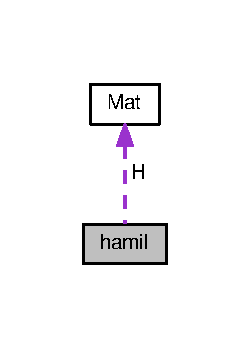
\includegraphics[width=120pt]{classhamil__coll__graph}
\end{center}
\end{figure}
\subsection*{Public Member Functions}
\begin{DoxyCompactItemize}
\item 
\hyperlink{classhamil_ad94d7476758c98d5b2af73f73d92e295}{hamil} (\hyperlink{classbasis}{basis} \&sector, double t, double U)
\item 
double \hyperlink{classhamil_a49c2202b93e45e07636a73679c62e55c}{ground\+\_\+state\+\_\+energy} ()
\item 
void \hyperlink{classhamil_a3e686a737e1019cea6dd3617065a7a7e}{diag} ()
\item 
complex$<$ double $>$ {\bfseries Greens\+\_\+function} (double, double)\hypertarget{classhamil_af3f1cab0e7c3a187df9b48de191c73ef}{}\label{classhamil_af3f1cab0e7c3a187df9b48de191c73ef}

\item 
void \hyperlink{classhamil_a607d29abc7e23f3097a546b1affa384b}{print\+\_\+hamil} ()
\item 
void \hyperlink{classhamil_ad0939704cbb18eaac49cce5961a28f9d}{print\+\_\+eigen} ()
\end{DoxyCompactItemize}
\subsection*{Public Attributes}
\begin{DoxyCompactItemize}
\item 
long \hyperlink{classhamil_a8f3ba91f36a6ef7cef1c2248668a9ba4}{n\+Hilbert}
\item 
unsigned \hyperlink{classhamil_ad69ef2d8298340ce7c49617f5ffc1b46}{seed}
\item 
\hyperlink{classMat}{Mat} \hyperlink{classhamil_aa440fff2dff9ec215fe5d50976deceae}{H}
\item 
std\+::vector$<$ double $>$ \hyperlink{classhamil_a22699c0dd6f460537289842e445d878e}{eigenvalues}
\item 
std\+::vector$<$ double $>$ \hyperlink{classhamil_a7626c19b1aebcf74f47a6ea77825d464}{psi\+\_\+0}
\item 
std\+::vector$<$ double $>$ \hyperlink{classhamil_ab301c39efac3bcbd0fa5df20be44643c}{psi\+\_\+n0}
\end{DoxyCompactItemize}


\subsection{Constructor \& Destructor Documentation}
\index{hamil@{hamil}!hamil@{hamil}}
\index{hamil@{hamil}!hamil@{hamil}}
\subsubsection[{\texorpdfstring{hamil(basis \&sector, double t, double U)}{hamil(basis &sector, double t, double U)}}]{\setlength{\rightskip}{0pt plus 5cm}hamil\+::hamil (
\begin{DoxyParamCaption}
\item[{{\bf basis} \&}]{sector, }
\item[{double}]{t, }
\item[{double}]{U}
\end{DoxyParamCaption}
)}\hypertarget{classhamil_ad94d7476758c98d5b2af73f73d92e295}{}\label{classhamil_ad94d7476758c98d5b2af73f73d92e295}
Initialize the hamiltonian matrix elements. 
\begin{DoxyParams}{Parameters}
{\em sector} & basis sector, \\
\hline
{\em t} & hopping strength, \\
\hline
{\em U} & onsite replusive interaction strength \\
\hline
\end{DoxyParams}


\subsection{Member Function Documentation}
\index{hamil@{hamil}!diag@{diag}}
\index{diag@{diag}!hamil@{hamil}}
\subsubsection[{\texorpdfstring{diag()}{diag()}}]{\setlength{\rightskip}{0pt plus 5cm}void hamil\+::diag (
\begin{DoxyParamCaption}
{}
\end{DoxyParamCaption}
)}\hypertarget{classhamil_a3e686a737e1019cea6dd3617065a7a7e}{}\label{classhamil_a3e686a737e1019cea6dd3617065a7a7e}
Diagonalize the full hamiltonian \index{hamil@{hamil}!ground\+\_\+state\+\_\+energy@{ground\+\_\+state\+\_\+energy}}
\index{ground\+\_\+state\+\_\+energy@{ground\+\_\+state\+\_\+energy}!hamil@{hamil}}
\subsubsection[{\texorpdfstring{ground\+\_\+state\+\_\+energy()}{ground_state_energy()}}]{\setlength{\rightskip}{0pt plus 5cm}double hamil\+::ground\+\_\+state\+\_\+energy (
\begin{DoxyParamCaption}
{}
\end{DoxyParamCaption}
)}\hypertarget{classhamil_a49c2202b93e45e07636a73679c62e55c}{}\label{classhamil_a49c2202b93e45e07636a73679c62e55c}
Return the ground state energy of the system \index{hamil@{hamil}!print\+\_\+eigen@{print\+\_\+eigen}}
\index{print\+\_\+eigen@{print\+\_\+eigen}!hamil@{hamil}}
\subsubsection[{\texorpdfstring{print\+\_\+eigen()}{print_eigen()}}]{\setlength{\rightskip}{0pt plus 5cm}void hamil\+::print\+\_\+eigen (
\begin{DoxyParamCaption}
{}
\end{DoxyParamCaption}
)}\hypertarget{classhamil_ad0939704cbb18eaac49cce5961a28f9d}{}\label{classhamil_ad0939704cbb18eaac49cce5961a28f9d}
Print the eigenvalues of the system \index{hamil@{hamil}!print\+\_\+hamil@{print\+\_\+hamil}}
\index{print\+\_\+hamil@{print\+\_\+hamil}!hamil@{hamil}}
\subsubsection[{\texorpdfstring{print\+\_\+hamil()}{print_hamil()}}]{\setlength{\rightskip}{0pt plus 5cm}void hamil\+::print\+\_\+hamil (
\begin{DoxyParamCaption}
{}
\end{DoxyParamCaption}
)}\hypertarget{classhamil_a607d29abc7e23f3097a546b1affa384b}{}\label{classhamil_a607d29abc7e23f3097a546b1affa384b}
Print the hamiltonian matrix 

\subsection{Member Data Documentation}
\index{hamil@{hamil}!eigenvalues@{eigenvalues}}
\index{eigenvalues@{eigenvalues}!hamil@{hamil}}
\subsubsection[{\texorpdfstring{eigenvalues}{eigenvalues}}]{\setlength{\rightskip}{0pt plus 5cm}std\+::vector$<$double$>$ hamil\+::eigenvalues}\hypertarget{classhamil_a22699c0dd6f460537289842e445d878e}{}\label{classhamil_a22699c0dd6f460537289842e445d878e}
Eigenvalues of the hamiltonian \index{hamil@{hamil}!H@{H}}
\index{H@{H}!hamil@{hamil}}
\subsubsection[{\texorpdfstring{H}{H}}]{\setlength{\rightskip}{0pt plus 5cm}{\bf Mat} hamil\+::H}\hypertarget{classhamil_aa440fff2dff9ec215fe5d50976deceae}{}\label{classhamil_aa440fff2dff9ec215fe5d50976deceae}
Hamiltonian matrix in C\+SR format \index{hamil@{hamil}!n\+Hilbert@{n\+Hilbert}}
\index{n\+Hilbert@{n\+Hilbert}!hamil@{hamil}}
\subsubsection[{\texorpdfstring{n\+Hilbert}{nHilbert}}]{\setlength{\rightskip}{0pt plus 5cm}long hamil\+::n\+Hilbert}\hypertarget{classhamil_a8f3ba91f36a6ef7cef1c2248668a9ba4}{}\label{classhamil_a8f3ba91f36a6ef7cef1c2248668a9ba4}
Size of the Hilbert space \index{hamil@{hamil}!psi\+\_\+0@{psi\+\_\+0}}
\index{psi\+\_\+0@{psi\+\_\+0}!hamil@{hamil}}
\subsubsection[{\texorpdfstring{psi\+\_\+0}{psi_0}}]{\setlength{\rightskip}{0pt plus 5cm}std\+::vector$<$double$>$ hamil\+::psi\+\_\+0}\hypertarget{classhamil_a7626c19b1aebcf74f47a6ea77825d464}{}\label{classhamil_a7626c19b1aebcf74f47a6ea77825d464}
Ground state wave function \index{hamil@{hamil}!psi\+\_\+n0@{psi\+\_\+n0}}
\index{psi\+\_\+n0@{psi\+\_\+n0}!hamil@{hamil}}
\subsubsection[{\texorpdfstring{psi\+\_\+n0}{psi_n0}}]{\setlength{\rightskip}{0pt plus 5cm}std\+::vector$<$double$>$ hamil\+::psi\+\_\+n0}\hypertarget{classhamil_ab301c39efac3bcbd0fa5df20be44643c}{}\label{classhamil_ab301c39efac3bcbd0fa5df20be44643c}
First element of all wave functions \index{hamil@{hamil}!seed@{seed}}
\index{seed@{seed}!hamil@{hamil}}
\subsubsection[{\texorpdfstring{seed}{seed}}]{\setlength{\rightskip}{0pt plus 5cm}unsigned hamil\+::seed}\hypertarget{classhamil_ad69ef2d8298340ce7c49617f5ffc1b46}{}\label{classhamil_ad69ef2d8298340ce7c49617f5ffc1b46}
seed for the R\+N\+Gs 

The documentation for this class was generated from the following files\+:\begin{DoxyCompactItemize}
\item 
hamiltonian.\+h\item 
hamiltonian.\+cpp\end{DoxyCompactItemize}

\hypertarget{classlhamil}{}\section{lhamil Class Reference}
\label{classlhamil}\index{lhamil@{lhamil}}


Collaboration diagram for lhamil\+:
\nopagebreak
\begin{figure}[H]
\begin{center}
\leavevmode
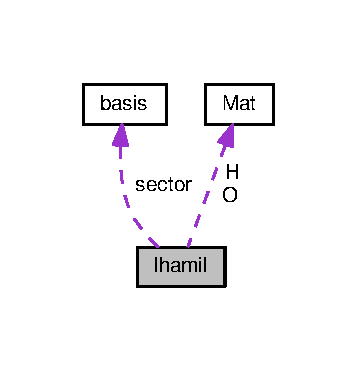
\includegraphics[width=172pt]{classlhamil__coll__graph}
\end{center}
\end{figure}
\subsection*{Public Member Functions}
\begin{DoxyCompactItemize}
\item 
{\bfseries lhamil} (const \hyperlink{classMat}{Mat} \&, long, long, unsigned)\hypertarget{classlhamil_a2ddee02e033269d368705a05fb14efd0}{}\label{classlhamil_a2ddee02e033269d368705a05fb14efd0}

\item 
{\bfseries lhamil} (\hyperlink{classbasis}{basis} \&, double, double, long, unsigned)\hypertarget{classlhamil_a250d9537be375f85843646cc1d31aed0}{}\label{classlhamil_a250d9537be375f85843646cc1d31aed0}

\item 
void {\bfseries set\+\_\+hamil} (\hyperlink{classbasis}{basis} \&, double, double)\hypertarget{classlhamil_a26e9de83711358c0ad92a19363eddb11}{}\label{classlhamil_a26e9de83711358c0ad92a19363eddb11}

\item 
void {\bfseries psir0\+\_\+creation\+\_\+el\+\_\+up} (\hyperlink{classbasis}{basis} \&, \hyperlink{classbasis}{basis} \&, vector$<$ double $>$ \&, long)\hypertarget{classlhamil_ad09d3c2f6fa1fad58e106815fef1e592}{}\label{classlhamil_ad09d3c2f6fa1fad58e106815fef1e592}

\item 
void {\bfseries psir0\+\_\+creation\+\_\+el\+\_\+down} (\hyperlink{classbasis}{basis} \&, \hyperlink{classbasis}{basis} \&, vector$<$ double $>$ \&, long)\hypertarget{classlhamil_af02ba60d0b23bca49ae084a810243357}{}\label{classlhamil_af02ba60d0b23bca49ae084a810243357}

\item 
void {\bfseries psir0\+\_\+annihilation\+\_\+el\+\_\+up} (\hyperlink{classbasis}{basis} \&, \hyperlink{classbasis}{basis} \&, vector$<$ double $>$ \&, long)\hypertarget{classlhamil_ac92fecae2024da4c02ac2d257b70dacb}{}\label{classlhamil_ac92fecae2024da4c02ac2d257b70dacb}

\item 
void {\bfseries psir0\+\_\+annihilation\+\_\+el\+\_\+down} (\hyperlink{classbasis}{basis} \&, \hyperlink{classbasis}{basis} \&, vector$<$ double $>$ \&, long)\hypertarget{classlhamil_ac3062ae288f9e6edcb0ebe322490fe55}{}\label{classlhamil_ac3062ae288f9e6edcb0ebe322490fe55}

\item 
void {\bfseries set\+\_\+onsite\+\_\+optc} (int r, int alpha, int annil)\hypertarget{classlhamil_a08c5ae8976b11b4673259d7b5e09ebcb}{}\label{classlhamil_a08c5ae8976b11b4673259d7b5e09ebcb}

\item 
void {\bfseries coeff\+\_\+update} ()\hypertarget{classlhamil_a57ef80505dfd7819444cc86e0f37b640}{}\label{classlhamil_a57ef80505dfd7819444cc86e0f37b640}

\item 
void {\bfseries coeff\+\_\+explicit\+\_\+update} ()\hypertarget{classlhamil_a747a5dbb742049be4057c3094fd1dffd}{}\label{classlhamil_a747a5dbb742049be4057c3094fd1dffd}

\item 
void {\bfseries coeff\+\_\+update\+\_\+wopt} (vector$<$ double $>$)\hypertarget{classlhamil_ae04b05c533b0f5fc91dd7ea12075a825}{}\label{classlhamil_ae04b05c533b0f5fc91dd7ea12075a825}

\item 
void {\bfseries diag} ()\hypertarget{classlhamil_ac9af1b00fc91983e100669171b02b708}{}\label{classlhamil_ac9af1b00fc91983e100669171b02b708}

\item 
void {\bfseries diag} (int)\hypertarget{classlhamil_a4c5ee9488fea26da2f6020063e8aeccf}{}\label{classlhamil_a4c5ee9488fea26da2f6020063e8aeccf}

\item 
void {\bfseries eigenstates\+\_\+reconstruction} ()\hypertarget{classlhamil_a8c7fce044a5ce803417ee685915f8bce}{}\label{classlhamil_a8c7fce044a5ce803417ee685915f8bce}

\item 
double {\bfseries ground\+\_\+state\+\_\+energy} ()\hypertarget{classlhamil_ada058bf85a90c1a1073aedda8303e942}{}\label{classlhamil_ada058bf85a90c1a1073aedda8303e942}

\item 
double {\bfseries spectral\+\_\+function} (double omega, double eta)\hypertarget{classlhamil_a6ac0b9160a5c8e9f55c1df2a4bc6b565}{}\label{classlhamil_a6ac0b9160a5c8e9f55c1df2a4bc6b565}

\item 
double {\bfseries spectral\+\_\+function} (double omega, double eta, int annil)\hypertarget{classlhamil_ae49314d086ae17932c1807904c5507bd}{}\label{classlhamil_ae49314d086ae17932c1807904c5507bd}

\item 
complex$<$ double $>$ {\bfseries Greens\+\_\+function} (double omega, double eta, int annil)\hypertarget{classlhamil_a657968fcec5a5231726184b2817eb8f6}{}\label{classlhamil_a657968fcec5a5231726184b2817eb8f6}

\item 
complex$<$ double $>$ {\bfseries Greens\+\_\+function\+\_\+ij\+\_\+ab} (int i, int j, int alpha, int beta, double E, double eta)\hypertarget{classlhamil_a02cb040876fa597d0e13486a0c7cfb73}{}\label{classlhamil_a02cb040876fa597d0e13486a0c7cfb73}

\item 
complex$<$ double $>$ {\bfseries Greens\+\_\+function\+\_\+k} (int k, int alpha, int beta, double E, double eta)\hypertarget{classlhamil_a22e29163bcb08ab415f3814490926d5c}{}\label{classlhamil_a22e29163bcb08ab415f3814490926d5c}

\item 
void {\bfseries print\+\_\+hamil} ()\hypertarget{classlhamil_ad4fb3d36c5dc5def8509f0a26d400579}{}\label{classlhamil_ad4fb3d36c5dc5def8509f0a26d400579}

\item 
void {\bfseries print\+\_\+lhamil} (int)\hypertarget{classlhamil_ab68145bc253a27018f0ff75b80a3d230}{}\label{classlhamil_ab68145bc253a27018f0ff75b80a3d230}

\item 
void {\bfseries print\+\_\+eigen} (int)\hypertarget{classlhamil_a2c26e7bbd48b2d7f46309508fc99854e}{}\label{classlhamil_a2c26e7bbd48b2d7f46309508fc99854e}

\item 
void {\bfseries save\+\_\+to\+\_\+file} (const char $\ast$)\hypertarget{classlhamil_adf3f7541e5922c3a6f03456edf924d1b}{}\label{classlhamil_adf3f7541e5922c3a6f03456edf924d1b}

\item 
void {\bfseries read\+\_\+from\+\_\+file} (const char $\ast$)\hypertarget{classlhamil_a0486bea26b7fc3c7544f75f3b70caa3e}{}\label{classlhamil_a0486bea26b7fc3c7544f75f3b70caa3e}

\end{DoxyCompactItemize}
\subsection*{Public Attributes}
\begin{DoxyCompactItemize}
\item 
unsigned {\bfseries seed}\hypertarget{classlhamil_a403c4979c8c75a247d526a88ad237d73}{}\label{classlhamil_a403c4979c8c75a247d526a88ad237d73}

\item 
long {\bfseries n\+Hilbert}\hypertarget{classlhamil_a4196bb19140860780faa0227b2b2d9d5}{}\label{classlhamil_a4196bb19140860780faa0227b2b2d9d5}

\item 
long {\bfseries lambda}\hypertarget{classlhamil_a19fc0f14305488a0f250b0e6e6541a32}{}\label{classlhamil_a19fc0f14305488a0f250b0e6e6541a32}

\item 
double {\bfseries E0}\hypertarget{classlhamil_a83f32edb3593b382e2cb3e469d95025e}{}\label{classlhamil_a83f32edb3593b382e2cb3e469d95025e}

\item 
std\+::vector$<$ double $>$ {\bfseries norm}\hypertarget{classlhamil_ae1e5cf1878aea2198372f64cd038ccc8}{}\label{classlhamil_ae1e5cf1878aea2198372f64cd038ccc8}

\item 
std\+::vector$<$ double $>$ {\bfseries overlap}\hypertarget{classlhamil_ab312761bed0e3f65e7143e06339e0773}{}\label{classlhamil_ab312761bed0e3f65e7143e06339e0773}

\item 
std\+::vector$<$ double $>$ {\bfseries psir\+\_\+0}\hypertarget{classlhamil_a30af2fba8c46ff87ec1144986321de93}{}\label{classlhamil_a30af2fba8c46ff87ec1144986321de93}

\item 
std\+::vector$<$ double $>$ {\bfseries psi\+\_\+0}\hypertarget{classlhamil_ad46e5575cd78453a79a4960d8f050708}{}\label{classlhamil_ad46e5575cd78453a79a4960d8f050708}

\item 
std\+::vector$<$ double $>$ {\bfseries psi\+\_\+n0}\hypertarget{classlhamil_a8380f1d9b7b9e819b43da1f374cc86b4}{}\label{classlhamil_a8380f1d9b7b9e819b43da1f374cc86b4}

\item 
std\+::vector$<$ double $>$ {\bfseries eigenvalues}\hypertarget{classlhamil_ae80fe2a6e59632516505e834f64053f2}{}\label{classlhamil_ae80fe2a6e59632516505e834f64053f2}

\item 
\hyperlink{classbasis}{basis} {\bfseries sector}\hypertarget{classlhamil_a3a5ef09836b4d5a13a6ff3aa62c67036}{}\label{classlhamil_a3a5ef09836b4d5a13a6ff3aa62c67036}

\item 
\hyperlink{classMat}{Mat} {\bfseries H}\hypertarget{classlhamil_af5eb4f55cd465808850890273b07d16a}{}\label{classlhamil_af5eb4f55cd465808850890273b07d16a}

\item 
\hyperlink{classMat}{Mat} {\bfseries O}\hypertarget{classlhamil_afa93e49df6f87889602b9fd4e84c511f}{}\label{classlhamil_afa93e49df6f87889602b9fd4e84c511f}

\end{DoxyCompactItemize}


The documentation for this class was generated from the following files\+:\begin{DoxyCompactItemize}
\item 
lanczos\+\_\+hamiltonian.\+h\item 
lanczos\+\_\+hamiltonian.\+cpp\end{DoxyCompactItemize}

\hypertarget{classMat}{}\section{Mat Class Reference}
\label{classMat}\index{Mat@{Mat}}
\subsection*{Public Member Functions}
\begin{DoxyCompactItemize}
\item 
{\bfseries Mat} (const \hyperlink{classMat}{Mat} \&rhs)\hypertarget{classMat_a689281bd62fd71097b8918a474baa03c}{}\label{classMat_a689281bd62fd71097b8918a474baa03c}

\item 
\hyperlink{classMat}{Mat} \& {\bfseries operator=} (const \hyperlink{classMat}{Mat} \&rhs)\hypertarget{classMat_ac5b996c2119fd4dfbcca681783471d06}{}\label{classMat_ac5b996c2119fd4dfbcca681783471d06}

\item 
\hyperlink{classVec}{Vec} {\bfseries operator$\ast$} (const \hyperlink{classVec}{Vec} \&) const \hypertarget{classMat_a96feace30905a807d746874106a917f1}{}\label{classMat_a96feace30905a807d746874106a917f1}

\item 
vector$<$ double $>$ {\bfseries operator$\ast$} (const vector$<$ double $>$ \&) const \hypertarget{classMat_a3c304227fd231e496d645522db714b5a}{}\label{classMat_a3c304227fd231e496d645522db714b5a}

\item 
void {\bfseries init} (const vector$<$ long $>$ \&, const vector$<$ long $>$ \&, const vector$<$ double $>$ \&)\hypertarget{classMat_a49db8fb674f8dd5f76bb6f7c710fa125}{}\label{classMat_a49db8fb674f8dd5f76bb6f7c710fa125}

\item 
void {\bfseries clear} ()\hypertarget{classMat_afccb6843f949660582b77cf677c7aee2}{}\label{classMat_afccb6843f949660582b77cf677c7aee2}

\item 
void {\bfseries print} ()\hypertarget{classMat_ab44133772f822f6963924b1a6e94290a}{}\label{classMat_ab44133772f822f6963924b1a6e94290a}

\end{DoxyCompactItemize}
\subsection*{Public Attributes}
\begin{DoxyCompactItemize}
\item 
std\+::vector$<$ long $>$ {\bfseries outer\+\_\+starts}\hypertarget{classMat_a4d8c91151fc8798ffe37835a6007e2f3}{}\label{classMat_a4d8c91151fc8798ffe37835a6007e2f3}

\item 
std\+::vector$<$ long $>$ {\bfseries inner\+\_\+indices}\hypertarget{classMat_adcb83b38680b48f2d29302e204294d79}{}\label{classMat_adcb83b38680b48f2d29302e204294d79}

\item 
std\+::vector$<$ double $>$ {\bfseries value}\hypertarget{classMat_a2c02c17a5641602e08ac5071a5c7da72}{}\label{classMat_a2c02c17a5641602e08ac5071a5c7da72}

\end{DoxyCompactItemize}


The documentation for this class was generated from the following files\+:\begin{DoxyCompactItemize}
\item 
matrix.\+h\item 
matrix.\+cpp\end{DoxyCompactItemize}

\hypertarget{classTimer}{}\section{Timer Class Reference}
\label{classTimer}\index{Timer@{Timer}}
\subsection*{Public Member Functions}
\begin{DoxyCompactItemize}
\item 
double {\bfseries elapsed} ()\hypertarget{classTimer_a7a0f15257db9fa349a43042d3d28349b}{}\label{classTimer_a7a0f15257db9fa349a43042d3d28349b}

\item 
unsigned long {\bfseries nanoseconds} ()\hypertarget{classTimer_a8e055136a144144d39628b64512b9067}{}\label{classTimer_a8e055136a144144d39628b64512b9067}

\item 
void {\bfseries reset} ()\hypertarget{classTimer_a9020542d73357a4eef512eefaf57524b}{}\label{classTimer_a9020542d73357a4eef512eefaf57524b}

\end{DoxyCompactItemize}


The documentation for this class was generated from the following file\+:\begin{DoxyCompactItemize}
\item 
init.\+h\end{DoxyCompactItemize}

\hypertarget{classVec}{}\section{Vec Class Reference}
\label{classVec}\index{Vec@{Vec}}
\subsection*{Public Member Functions}
\begin{DoxyCompactItemize}
\item 
{\bfseries Vec} (long \+\_\+size)\hypertarget{classVec_aebab4a32b6fd890bac3bb4ac0803000a}{}\label{classVec_aebab4a32b6fd890bac3bb4ac0803000a}

\item 
{\bfseries Vec} (long \+\_\+size, const double \+\_\+init)\hypertarget{classVec_a677cce187b9cdd48f87bb114e96a7f18}{}\label{classVec_a677cce187b9cdd48f87bb114e96a7f18}

\item 
{\bfseries Vec} (const \hyperlink{classVec}{Vec} \&rhs)\hypertarget{classVec_a81909697772bb0c9c21e84563118fd5e}{}\label{classVec_a81909697772bb0c9c21e84563118fd5e}

\item 
void {\bfseries assign} (long \+\_\+size, const double \+\_\+init)\hypertarget{classVec_a120192dd81c707083c3579372ea47bed}{}\label{classVec_a120192dd81c707083c3579372ea47bed}

\item 
void {\bfseries init\+\_\+random} (unsigned)\hypertarget{classVec_aa0d1a2202064a2b55efe1bdf5c6cab29}{}\label{classVec_aa0d1a2202064a2b55efe1bdf5c6cab29}

\item 
void {\bfseries init\+\_\+random} (long, unsigned)\hypertarget{classVec_aee89a807828fa09404834adb1f5507b0}{}\label{classVec_aee89a807828fa09404834adb1f5507b0}

\item 
void {\bfseries clear} ()\hypertarget{classVec_a3d89cd4aa378073a229f7bc6eb2b40b2}{}\label{classVec_a3d89cd4aa378073a229f7bc6eb2b40b2}

\item 
double {\bfseries normalize} ()\hypertarget{classVec_a22d5787f88ef4a6ead33c0857d3da697}{}\label{classVec_a22d5787f88ef4a6ead33c0857d3da697}

\item 
\hyperlink{classVec}{Vec} \& {\bfseries operator=} (const \hyperlink{classVec}{Vec} \&rhs)\hypertarget{classVec_a2432e72a4c830d7ae40d36fe843f8fa0}{}\label{classVec_a2432e72a4c830d7ae40d36fe843f8fa0}

\item 
\hyperlink{classVec}{Vec} \& {\bfseries operator-\/=} (const \hyperlink{classVec}{Vec} \&rhs)\hypertarget{classVec_adce31c56c9f71357dfea84f44e461d0c}{}\label{classVec_adce31c56c9f71357dfea84f44e461d0c}

\item 
\hyperlink{classVec}{Vec} \& {\bfseries operator+=} (const \hyperlink{classVec}{Vec} \&rhs)\hypertarget{classVec_aa5147cd7b8bbfde4d9cfe50c5ef06d0e}{}\label{classVec_aa5147cd7b8bbfde4d9cfe50c5ef06d0e}

\item 
\hyperlink{classVec}{Vec} \& {\bfseries operator$\ast$=} (const double \&rhs)\hypertarget{classVec_a1d19c62e25c778f17c57825979fdb774}{}\label{classVec_a1d19c62e25c778f17c57825979fdb774}

\item 
\hyperlink{classVec}{Vec} \& {\bfseries operator/=} (const double \&rhs)\hypertarget{classVec_afef031c2f4974301a8ebb4488eb7ba67}{}\label{classVec_afef031c2f4974301a8ebb4488eb7ba67}

\item 
\hyperlink{classVec}{Vec} {\bfseries operator+} (const \hyperlink{classVec}{Vec} \&)\hypertarget{classVec_acb13469c3a3644e1abf1ee519553ff56}{}\label{classVec_acb13469c3a3644e1abf1ee519553ff56}

\item 
\hyperlink{classVec}{Vec} {\bfseries operator-\/} (const \hyperlink{classVec}{Vec} \&)\hypertarget{classVec_a005a4aa5f7dae6324715187ddd650138}{}\label{classVec_a005a4aa5f7dae6324715187ddd650138}

\item 
\hyperlink{classVec}{Vec} {\bfseries operator$\ast$} (const double \&)\hypertarget{classVec_a9b6a01d2684968405d122f6b6c6051f9}{}\label{classVec_a9b6a01d2684968405d122f6b6c6051f9}

\item 
\hyperlink{classVec}{Vec} {\bfseries operator/} (const double \&)\hypertarget{classVec_a0fbd49c62772e5078e181f97265baf6f}{}\label{classVec_a0fbd49c62772e5078e181f97265baf6f}

\item 
double {\bfseries operator$\ast$} (const \hyperlink{classVec}{Vec} \&)\hypertarget{classVec_ac9421c042b0c2e0cbfd92ffa46608d96}{}\label{classVec_ac9421c042b0c2e0cbfd92ffa46608d96}

\end{DoxyCompactItemize}
\subsection*{Public Attributes}
\begin{DoxyCompactItemize}
\item 
std\+::vector$<$ double $>$ {\bfseries value}\hypertarget{classVec_a84e5d0f3dfe0e0a1ad564da467b3615c}{}\label{classVec_a84e5d0f3dfe0e0a1ad564da467b3615c}

\item 
long {\bfseries size}\hypertarget{classVec_a141b4ba2dd3195c5cb28f19297e77468}{}\label{classVec_a141b4ba2dd3195c5cb28f19297e77468}

\end{DoxyCompactItemize}
\subsection*{Friends}
\begin{DoxyCompactItemize}
\item 
ostream \& {\bfseries operator$<$$<$} (ostream \&os, const \hyperlink{classVec}{Vec} \&)\hypertarget{classVec_a2f626ba27f64fc7f61dfe6dcefa5a08e}{}\label{classVec_a2f626ba27f64fc7f61dfe6dcefa5a08e}

\end{DoxyCompactItemize}


The documentation for this class was generated from the following files\+:\begin{DoxyCompactItemize}
\item 
matrix.\+h\item 
matrix.\+cpp\end{DoxyCompactItemize}

%--- End generated contents ---

% Index
\backmatter
\newpage
\phantomsection
\clearemptydoublepage
\addcontentsline{toc}{chapter}{Index}
\printindex

\end{document}
